\documentclass[10pt]{article}

% Page layout
\usepackage[margin=0.9in]{geometry}
\usepackage[T1]{fontenc}
\usepackage{lmodern}

% Math, tables, figures, lists
\usepackage{amsmath,amssymb}
\usepackage{booktabs}
\usepackage{graphicx}
\usepackage{enumitem}
\usepackage{placeins}
\setlist{nosep,leftmargin=*}

% Citations and links
\usepackage[numbers,sort&compress]{natbib}
\usepackage[hidelinks]{hyperref}

\title{How Well Do Tuned Neural CATE Estimators Transfer?\\
TARNet and DragonNet on IHDP and Controlled Synthetic Data}
\author{Disha Sharma\\
Gautam Buddha University, Greater Noida, India}
\date{}

\begin{document}
\maketitle

\begin{abstract}
Neural networks are a common approach to estimating individual treatment effects, but comparisons with tree-based estimators are sensitive to hyperparameter tuning and to the benchmark used. We compare TARNet and DragonNet, implemented in PyTorch, with a T-learner, a causal forest and a linear double machine learning estimator on the IHDP benchmark and on a synthetic benchmark with controlled effect heterogeneity and confounding strength. All tuning uses IHDP replications 0--19, configurations are frozen, and the final comparison uses held-out replications 20--99. On held-out IHDP, tuned TARNet and DragonNet have mean in-sample $\sqrt{\mathrm{PEHE}}$ of 0.82 and 0.90, against 1.97 for the T-learner and 3.41 for the causal forest, and TARNet has lower error than the T-learner in 79 of 80 replications. DragonNet's propensity head and targeted regularisation improve on the same network without them, but we find no consistent advantage over TARNet. On synthetic data, however, the settings tuned on IHDP are worse than default settings at moderate and high heterogeneity in every seed, and a sensitivity analysis points to weight decay as the main cause. The causal forest is competitive only when true effects are nearly constant. Our results suggest that hyperparameters tuned on one benchmark should not be assumed to transfer to data with a different effect scale.
\end{abstract}

\section{Introduction}

Estimating how the effect of a treatment varies across individuals, the conditional average treatment effect (CATE), is central to personalised decisions in education, medicine and marketing. With observational data the estimate must also adjust for confounding, and the error of interest is the error on individual effects, not only on their average.

Neural estimators are a common approach. TARNet \citep{shalit2017estimating} learns a shared representation of the covariates that feeds two outcome heads, one per treatment arm, and DragonNet \citep{shi2019adapting} adds a propensity-score head and a targeted-regularisation term on the same representation. Tree-based and residual-based alternatives include causal forests \citep{wager2018estimation}, double machine learning \citep{chernozhukov2018double} and meta-learners such as the T-learner \citep{kunzel2019metalearners}; the first two are available in the EconML package \citep{battocchi2019econml}. Reported rankings of CATE estimators can depend on the benchmark used \citep{curth2021really}.

We study this on the IHDP benchmark \citep{hill2011bayesian}, using the standard 100 simulated replications \citep{shalit2017estimating}, and on a synthetic benchmark in which we control effect heterogeneity and confounding strength. We ask three questions:
\begin{enumerate}
  \item With a tuning protocol fixed before the final evaluation, how do tuned TARNet and DragonNet compare with a tuned T-learner and a tuned causal forest on held-out IHDP replications?
  \item Do DragonNet's propensity head and targeted regularisation improve on the same network without them?
  \item Do hyperparameters tuned on IHDP transfer to data with different, controlled levels of heterogeneity and confounding?
\end{enumerate}

Our protocol uses IHDP replications 0--19 for all tuning, freezes every configuration, and reports the final comparison on replications 20--99 and on all 100, with paired per-replication tests. Our main findings are as follows. On held-out IHDP replications, tuned TARNet and DragonNet clearly outperform the tuned T-learner and causal forest. DragonNet's extra terms help relative to its own stripped version, but tuned TARNet matches or slightly outperforms tuned DragonNet. On synthetic data, the IHDP-tuned settings are worse than default settings at moderate and high heterogeneity, and a sensitivity analysis points to weight decay as the main cause. The forest baseline is competitive only when true effects are nearly constant.

\section{Methods}

\subsection{Data}

\textbf{IHDP.} We use the standard 100-replication version of the semi-synthetic IHDP benchmark \citep{hill2011bayesian,shalit2017estimating}. Each replication has 25 covariates, a binary treatment and a simulated outcome, and the potential-outcome means are available, so true individual effects are known. Each replication has 672 training units and 75 test units.

\textbf{Synthetic benchmark.} Covariates are $X\sim N(0,I_{10})$, treatment is $T\sim\mathrm{Bernoulli}(e(X))$ and $Y=\mu_0(X)+T\,\tau(X)+\varepsilon$ with $\varepsilon\sim N(0,1)$, where
\begin{align}
\mu_0(x) &= 2x_1 + x_2 + 0.5x_3^2 + \sin(x_4),\\
\tau(x) &= 1 + h\,\frac{s(x)-\bar s}{\sigma_s}, \qquad s(x)=\tanh(x_1)+0.5\,x_2x_3+0.5\,\mathbf{1}[x_4>0],\\
e(x) &= \mathrm{clip}\!\left(\sigma\!\left(c\,(0.8x_1+0.5x_2-0.5x_3+0.3x_4)\right),\,0.05,\,0.95\right).
\end{align}
Here $\bar s$ and $\sigma_s$ are the mean and standard deviation of $s(X)$ estimated from a reference sample of 200{,}000 draws, so the true effects have standard deviation close to $h$ and an average close to 1. Heterogeneity $h\in\{0.5,2.5,8\}$ and confounding strength $c\in\{0.5,1.5\}$ define six cells. Each dataset has 2{,}000 training units and 500 test units with fresh covariates, and we run 10 seeds per cell. The baseline outcome and the treatment score share the same covariates, which creates confounding. Because $\tau$ also depends on those covariates, the bias of the naive difference in means grows with $h$ as well as with $c$, so the two axes are not fully independent.

\subsection{Estimators}

The \textbf{naive} baseline predicts the difference in mean outcomes between treated and control units for every unit. The \textbf{T-learner} fits one random forest regressor per treatment arm (200 trees, scikit-learn \citep{pedregosa2011scikit}) and takes the difference of their predictions. \textbf{LinearDML} and \textbf{CausalForestDML} are from EconML \citep{battocchi2019econml}, with random forest nuisance models (100 trees, minimum leaf size 5) for the outcome and for the discrete treatment. CausalForestDML uses 200 trees. LinearDML is not tuned.

\textbf{TARNet} has a shared representation of three fully connected ELU layers, followed by two outcome heads with two hidden layers of width 100, one per treatment arm. \textbf{DragonNet} has the same body and heads and adds a linear propensity head on the representation. Its loss is $\mathcal{L}=\mathcal{L}_{y}+\alpha\,\mathcal{L}_{e}+\beta\,\mathcal{L}_{\mathrm{targ}}$, with squared error on the factual outcome, binary cross-entropy for the propensity, and the targeted-regularisation term with a learnable $\epsilon$ and propensities clipped to $[0.01,0.99]$ \citep{shi2019adapting}; $\alpha=\beta=1$ unless stated. We implemented both networks in PyTorch \citep{paszke2019pytorch} and they may differ from the authors' reference implementations in training details.

Both networks are trained with Adam (learning rate $10^{-3}$, batch size 64, at most 300 epochs). Covariates and outcomes are standardised using training statistics. Weight decay is the L2 penalty in Adam. We hold out 20\% of the training units, stratified by treatment, and stop when the factual outcome loss on them has not improved for 20 epochs, keeping the best epoch. Stopping uses factual outcomes only. The random seed of each fit is the replication index (IHDP) or dataset seed (synthetic).

\subsection{Tuning protocol}

All tuning uses IHDP replications 0--19 only. Configurations are ranked by the median in-sample $\sqrt{\mathrm{PEHE}}$ across these replications, since means are dominated by a few replications with very large effects. Every selected configuration was saved before the held-out run, and the final comparison uses replications 20--99 and, separately, all 100. Selection uses the true effects, which are unavailable outside benchmarks, so held-out replications are needed for an unbiased comparison. Table~\ref{tab:configs} lists the frozen settings and the search budgets. The neural search started from weight decay in $\{10^{-4},10^{-3},10^{-2}\}$ crossed with widths $\{64,200\}$, and was extended in steps when the best configuration lay on the boundary, adding weight decays $3\times10^{-2}$ and $10^{-1}$ and widths 32 and 16. Not every combination was run. We capped the budget at 13 configurations, and the best widths are at the lower edge of the grid, so lower widths were not explored. The synthetic benchmark uses the IHDP-frozen configurations without retuning. We also report TARNet and DragonNet at default settings (weight decay $10^{-4}$, width 200) there.

\begin{table}[t]
\centering
\small
\caption{Configurations frozen on IHDP replications 0--19 and the number of configurations evaluated.}
\label{tab:configs}
\begin{tabular}{lll}
\toprule
Estimator & Frozen setting & Configurations tried \\
\midrule
T-learner & minimum leaf 3, max features 0.5 & 13 \\
CausalForestDML & minimum leaf 5, max samples 0.5 & 12 \\
TARNet & weight decay $10^{-2}$, width 16 & 13 \\
DragonNet & weight decay $3\times10^{-2}$, width 16 & 13 \\
\bottomrule
\end{tabular}
\end{table}

\subsection{Evaluation}

We report $\sqrt{\mathrm{PEHE}}=\sqrt{\tfrac1n\sum_i(\hat\tau(x_i)-\tau(x_i))^2}$ and the absolute ATE error, in-sample (training units) and out-of-sample (test units). Summaries give the mean with a 95\% confidence interval across replications (normal approximation on IHDP, $t$-based on the synthetic seeds) and the median. Comparisons between estimators use per-replication differences, with a two-sided sign test and a Wilcoxon signed-rank test on the 80 held-out IHDP replications. For the synthetic benchmark we report win counts over the 10 seeds per cell, without formal tests. All 100 IHDP replications use the same 747 units, with identical covariates and treatment assignment, so the tests describe variation across simulated outcomes and not across populations. We also stratify the IHDP replications into terciles of the standard deviation of the true effects, a post hoc analysis that we treat as exploratory.

All experiments ran on CPU in Google Colab with Python 3.13.15, PyTorch 2.11.0, scikit-learn 1.6.1 and EconML 0.17.0, together with NumPy 2.1.3, pandas 2.2.3 and SciPy 1.16.3. Re-running a fixed configuration with the same seeds reproduced our results.

\section{Results}

\subsection{IHDP: held-out replications}

Table~\ref{tab:ihdp} reports the frozen configurations on replications 20--99, which were not used for tuning. Tuned TARNet and DragonNet have far lower error than the tuned T-learner and causal forest, both in-sample and out-of-sample. In-sample $\sqrt{\mathrm{PEHE}}$ is 0.82 for TARNet and 0.90 for DragonNet, against 1.97 for the T-learner and 3.41 for CausalForestDML. Paired per-replication differences give the same picture: TARNet has lower error than the T-learner in 79 of 80 replications (median difference $-0.46$) and than CausalForestDML in 77 of 80 (median difference $-1.12$), and DragonNet beats them in 78 and 76 of 80. All four comparisons have two-sided sign-test and Wilcoxon $p<10^{-4}$. Means and medians differ widely for the baselines, because a few replications have very large true effects and dominate the means. For this reason we report medians alongside means throughout. Rankings on all 100 replications are the same as on the held-out 80 (TARNet mean 0.82, median 0.49; DragonNet mean 0.90, median 0.55).
For reference, TARNet at default settings (weight decay $10^{-4}$, width 200) had a mean $\sqrt{\mathrm{PEHE}}$ of 1.03 and a median of 0.92 over all 100 replications, against 0.82 and 0.49 when tuned.

\begin{table}[t]
\centering
\small
\caption{IHDP held-out replications 20--99: $\sqrt{\mathrm{PEHE}}$, mean $\pm$ 95\% confidence interval half-width, and median.}
\label{tab:ihdp}
\begin{tabular}{lcccc}
\toprule
 & \multicolumn{2}{c}{In-sample} & \multicolumn{2}{c}{Out-of-sample} \\
\cmidrule(lr){2-3}\cmidrule(lr){4-5}
Estimator & Mean $\pm$ CI & Median & Mean $\pm$ CI & Median \\
\midrule
Naive & $5.64 \pm 1.74$ & 2.70 & $5.74 \pm 1.88$ & 2.74 \\
LinearDML & $3.10 \pm 0.90$ & 1.50 & $3.16 \pm 0.92$ & 1.66 \\
CausalForestDML & $3.41 \pm 1.06$ & 1.61 & $3.60 \pm 1.23$ & 1.68 \\
T-learner & $1.97 \pm 0.59$ & 0.91 & $2.66 \pm 0.94$ & 1.18 \\
DragonNet & $0.90 \pm 0.20$ & 0.57 & $1.04 \pm 0.32$ & 0.59 \\
TARNet & $\mathbf{0.82 \pm 0.19}$ & \textbf{0.49} & $\mathbf{0.95 \pm 0.29}$ & \textbf{0.53} \\
\bottomrule
\end{tabular}
\end{table}

TARNet has lower error than DragonNet in 62 of 80 held-out replications (median difference $-0.06$, $p<10^{-4}$ for both tests), although the mean confidence intervals overlap. The two networks were tuned separately and ended with different weight decays (Table~\ref{tab:configs}), so this comparison does not isolate the effect of DragonNet's extra heads. The next subsection addresses that.

We stratified replications into terciles of the standard deviation of the true effects (a post hoc, exploratory analysis). Among the tuned models, both networks have lower median error than the T-learner and CausalForestDML in all three terciles: 0.35 (TARNet) and 0.34 (DragonNet) in the lowest tercile, against 0.55 for both the T-learner and CausalForestDML, and 1.04 (TARNet) and 1.25 (DragonNet) in the highest, against 2.84 (T-learner) and 5.44 (CausalForestDML). With all models at default settings (all 100 replications), the lowest tercile looked different: the median error of TARNet was 0.73 against 0.54 for both the T-learner and CausalForestDML. These two analyses use different replication sets and tuning states, so the contrast is descriptive and does not isolate the effect of tuning.

\subsection{Effect of DragonNet's propensity head and targeted regularisation}

To isolate the extra terms, we kept DragonNet's frozen configuration (weight decay $3\times10^{-2}$, width 16) and switched them off (Table~\ref{tab:ablation}). The full model has lower error than the variant with $\alpha=\beta=0$ in 59 of 80 held-out replications (median difference $-0.07$) and lower error than the propensity-only variant in 66 of 80 (median difference $-0.08$); both have $p<10^{-4}$. The propensity-only variant is indistinguishable from the stripped one (38 of 80 wins, $p=0.74$). The gain therefore appears only when the propensity head and the targeted term are combined. We did not run a variant with the targeted term and no propensity loss, since the propensity estimates would then be untrained, so we cannot separate their contributions further.

\begin{table}[t]
\centering
\small
\caption{DragonNet ablation on IHDP replications 20--99 (same weight decay and width). TARNet at its own frozen configuration is shown for reference.}
\label{tab:ablation}
\begin{tabular}{lcccc}
\toprule
 & \multicolumn{2}{c}{In-sample} & \multicolumn{2}{c}{Out-of-sample} \\
\cmidrule(lr){2-3}\cmidrule(lr){4-5}
Variant & Mean & Median & Mean & Median \\
\midrule
Full DragonNet & 0.90 & 0.57 & 1.04 & 0.59 \\
Propensity loss only ($\beta=0$) & 1.06 & 0.63 & 1.17 & 0.62 \\
No extra terms ($\alpha=\beta=0$) & 1.06 & 0.64 & 1.16 & 0.66 \\
TARNet (reference) & 0.82 & 0.49 & 0.95 & 0.53 \\
\bottomrule
\end{tabular}
\end{table}

\subsection{Synthetic benchmark}

Table~\ref{tab:synthetic} and Figure~\ref{fig:synthetic} show in-sample $\sqrt{\mathrm{PEHE}}$ over the six synthetic cells. Out-of-sample errors are within 0.12 of the in-sample errors in every cell for all estimators except the T-learner, whose largest gap is 0.52.

\begin{table}[t]
\centering
\footnotesize
\caption{Synthetic benchmark: mean in-sample $\sqrt{\mathrm{PEHE}}$ over 10 seeds. CF = CausalForestDML, T = T-learner, TAR-t / TAR-d = TARNet tuned / default, DN-t / DN-d = DragonNet tuned / default. Best per row in bold.}
\label{tab:synthetic}
\begin{tabular}{llcccccc}
\toprule
$h$ & $c$ & CF & T & TAR-t & TAR-d & DN-t & DN-d \\
\midrule
0.5 & 0.5 & \textbf{0.370} & 0.749 & 0.391 & 0.439 & 0.407 & 0.456 \\
0.5 & 1.5 & \textbf{0.420} & 1.014 & 0.454 & 0.498 & 0.557 & 0.513 \\
2.5 & 0.5 & 1.365 & 1.279 & 1.166 & \textbf{0.726} & 1.261 & 0.781 \\
2.5 & 1.5 & 1.418 & 1.673 & 1.233 & 0.791 & 1.266 & \textbf{0.785} \\
8.0 & 0.5 & 4.318 & 3.678 & 2.194 & \textbf{1.208} & 2.642 & 1.267 \\
8.0 & 1.5 & 4.306 & 3.940 & 2.622 & \textbf{1.359} & 2.739 & 1.509 \\
\bottomrule
\end{tabular}
\end{table}

\begin{figure}[t]
\centering
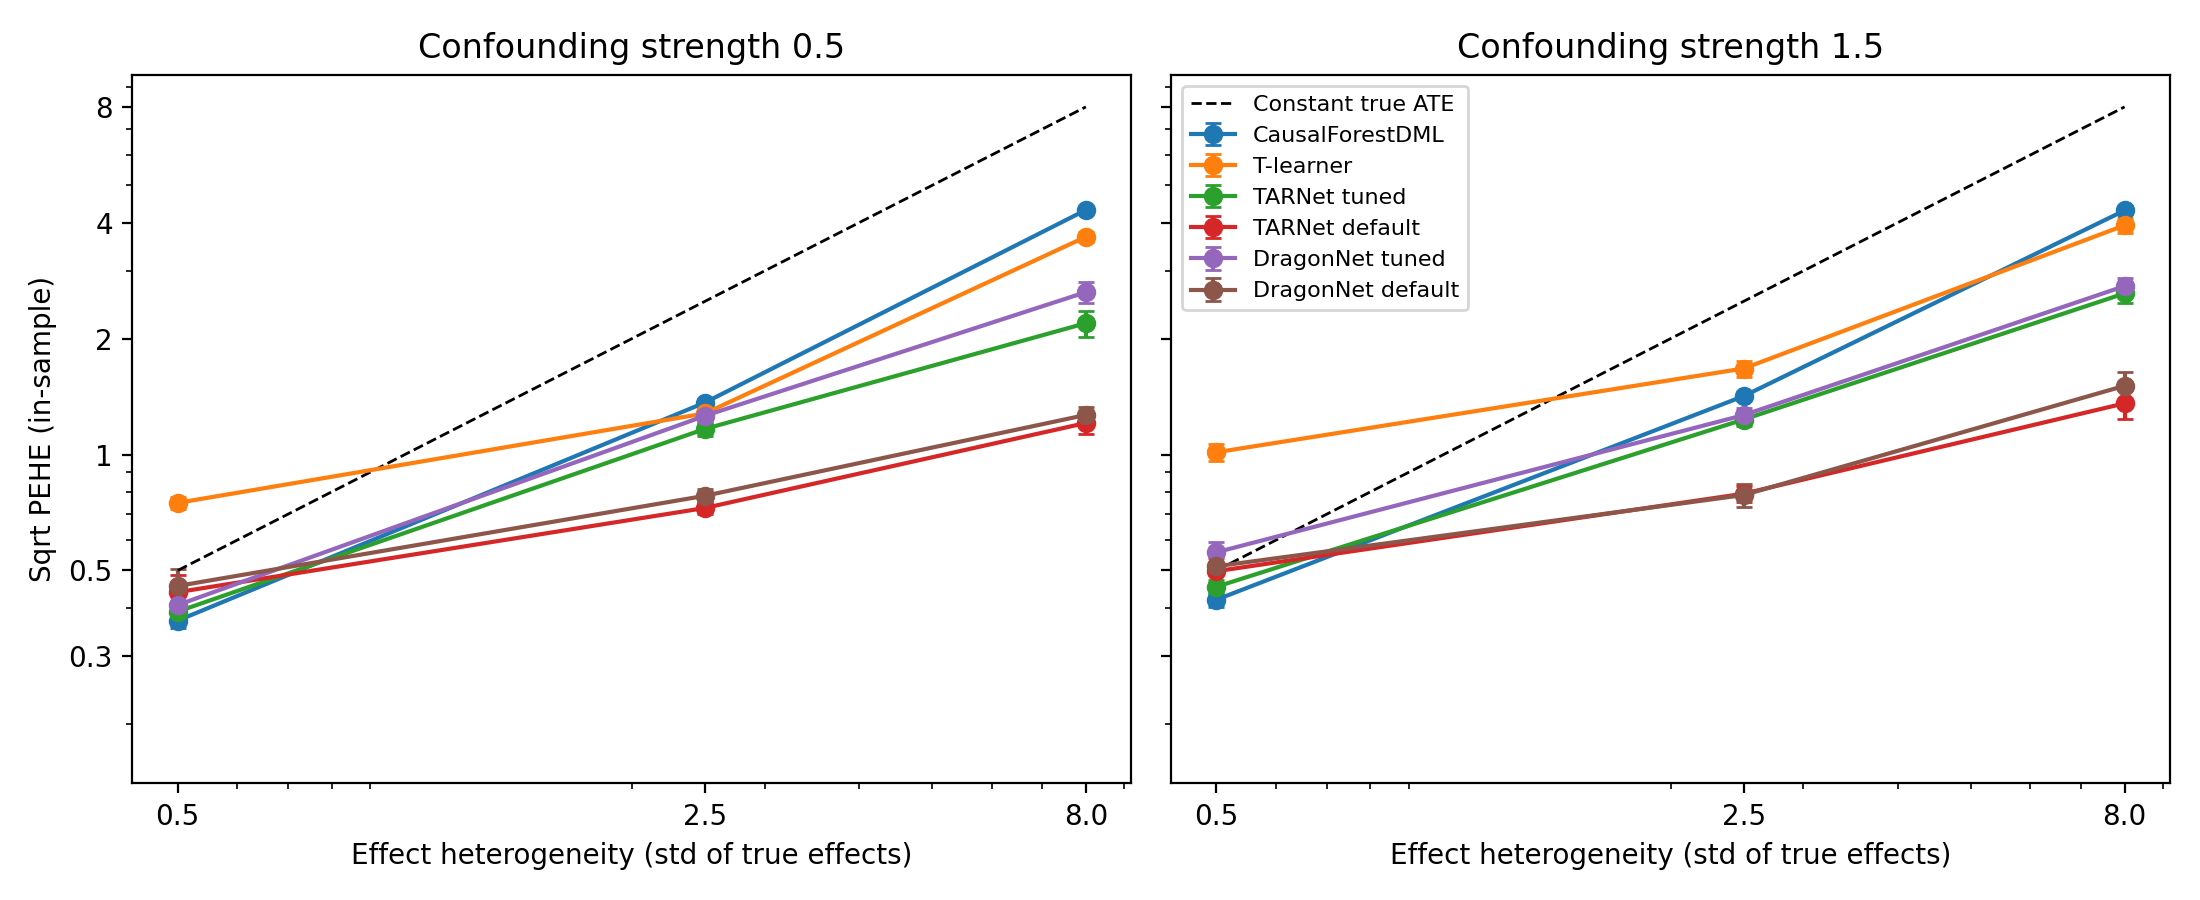
\includegraphics[width=\linewidth]{synthetic_pehe_vs_het.png}
\caption{Mean in-sample $\sqrt{\mathrm{PEHE}}$ against effect heterogeneity for the two confounding levels (10 seeds; bars are 95\% $t$-intervals). The dashed line is the error of predicting the true average effect for every unit, which is approximately $h$.}
\label{fig:synthetic}
\end{figure}

\textbf{Heterogeneity and the forest baseline.} At $h=0.5$, CausalForestDML has the lowest mean error (0.37 and 0.42), tuned TARNet is close behind (0.39 and 0.45), and default TARNet is worse, losing to the forest in 9 and 10 of 10 seeds. At $h=2.5$ and $h=8$, both TARNet versions have lower error than the forest in all 10 seeds in all four cells. Where $h=8$, the forest's error (about 4.3) is more than three times that of default TARNet (1.2 and 1.4). The T-learner has higher error than CausalForestDML at $h=0.5$ in both confounding settings (0.75 and 1.01 against 0.37 and 0.42) and its error exceeds $h$ there, so a constant prediction at the true average effect would have done better.

\textbf{Tuned versus default networks.} Settings tuned on IHDP do not transfer. At $h=2.5$ and $h=8$, tuned TARNet and tuned DragonNet have higher error than their default versions in all 10 seeds in all eight comparisons, with mean gaps of 0.44 to 1.37. At $h=0.5$ the tuned versions are slightly better for TARNet (8 and 7 of 10 seeds, mean gaps of about 0.05) and mixed for DragonNet (7 and 3 of 10).

\textbf{DragonNet versus TARNet.} At default settings, DragonNet's mean error is higher than TARNet's in five of the six cells (by 0.015 to 0.150) and lower in one (by 0.006). In the five cells where it is higher, DragonNet has lower error in at most 3 of 10 seeds. In the sixth cell it has lower error in 8 of 10 seeds, which is not significant (two-sided sign test $p=0.11$).

\textbf{Confounding strength.} Raising $c$ from 0.5 to 1.5 increases the error of the T-learner in every row ($+0.26$ to $+0.39$). Default TARNet changes less ($+0.06$ to $+0.15$) and CausalForestDML hardly changes.

\subsection{Sensitivity to weight decay and width}

To see which hyperparameter drives the loss of the tuned networks, we ran TARNet at $h=8$, $c=1.5$ over several settings (Table~\ref{tab:sens}). This analysis was run after the main comparison, and it did not affect any selection. At fixed width 200, error rises steadily with weight decay (1.36, 1.60, 2.63 and 3.21 for $10^{-4}$, $10^{-3}$, $10^{-2}$ and $3\times10^{-2}$). At fixed weight decay $10^{-4}$, narrowing the representation raises the error much less (1.36, 1.41 and 1.73 for widths 200, 64 and 16). At weight decay $10^{-2}$, width 16 and width 200 give almost the same error (2.62 and 2.63). In this cell, therefore, the weight decay chosen on IHDP accounts for most of the gap to the default. We did not test why large weight decay hurts here, and we ran the analysis only for TARNet in one cell.

\begin{table}[t]
\centering
\small
\caption{TARNet sensitivity at $h=8$, $c=1.5$ (mean in-sample $\sqrt{\mathrm{PEHE}}$, 10 seeds).}
\label{tab:sens}
\begin{tabular}{llc}
\toprule
Weight decay & Width & $\sqrt{\mathrm{PEHE}}$ \\
\midrule
$10^{-4}$ & 200 (default) & 1.359 \\
$10^{-4}$ & 64 & 1.413 \\
$10^{-4}$ & 16 & 1.729 \\
$10^{-3}$ & 200 & 1.602 \\
$10^{-2}$ & 200 & 2.633 \\
$3\times10^{-2}$ & 200 & 3.209 \\
$10^{-2}$ & 16 (tuned) & 2.622 \\
\bottomrule
\end{tabular}
\end{table}

\section{Discussion}

\textbf{Tuned networks on IHDP.} On the held-out replications, tuned TARNet and DragonNet had much lower error than the tuned T-learner and causal forest, and won 76 to 79 of 80 paired comparisons. Tuning accounts for part of this advantage. Over all 100 replications, TARNet's median in-sample $\sqrt{\mathrm{PEHE}}$ fell from 0.92 at default settings to 0.49 when tuned (the tuned figure includes the 20 tuning replications, but is the same on the held-out 80). Where effects were nearly constant, the tree-based methods led at default settings on all 100 replications, while the tuned networks had lower median error in every tercile of the held-out replications.

\textbf{Tuning did not transfer.} The weight decay that helped on IHDP hurt on synthetic data with larger effects: at $h=2.5$ and $h=8$, the tuned networks had higher error than the default ones in every seed. A sensitivity analysis in one cell points to weight decay, not width, as the main cause. One possible explanation is that strong shrinkage limits how large an effect surface the outcome heads can represent, but we did not test this. The practical point is that hyperparameters chosen on one benchmark should not be assumed to carry over to data with a different effect scale. Real applications also need selection criteria that do not require the true effects, which our protocol used on the development replications.

\textbf{Forest baseline.} CausalForestDML had the lowest error when effects were nearly constant ($h=0.5$), but its error grew by a factor of about 12 as $h$ rose from 0.5 to 8 ($c=0.5$), while default TARNet's grew by a factor of under 3. We have only three heterogeneity levels, so this is a description of our grid, not a fitted scaling law.

\textbf{DragonNet.} On IHDP, the propensity head and targeted-regularisation term improved DragonNet relative to the same network without them, and the gain appeared only when both were present. We found no consistent advantage over TARNet on either benchmark, and no sign on the synthetic data that the propensity head helps more under stronger confounding.

\section{Limitations}

\begin{itemize}
  \item \textbf{Replications are not independent.} All 100 IHDP replications use the same 747 units, with identical covariates and treatment assignment, so the paired tests describe variation across simulated outcomes, not across populations. The synthetic cells reuse seeds across cells.
  \item \textbf{One synthetic design.} We used a single effect-surface shape, $n=2{,}000$ and 10 covariates. Heterogeneity and confounding are coupled, because the effect depends on the covariates that drive treatment.
  \item \textbf{Asymmetric search.} The neural networks were tuned over weight decay and representation width only. Learning rate, depth, head width and batch size were fixed. The forest and T-learner searches covered leaf size and a subsampling fraction, with the number of trees and the nuisance models fixed, and LinearDML was not tuned. The best neural widths lie at the lower edge of the grid.
  \item \textbf{Oracle selection.} Configurations were chosen using the true individual effects on the development replications, which are unavailable outside benchmarks.
  \item \textbf{Own implementations.} Our TARNet has no balancing penalty, and our PyTorch implementations of both networks may differ from the reference implementations in training details. We did not verify parity.
  \item \textbf{Exploratory analyses.} The effect-spread terciles and the weight-decay sensitivity analysis were run after seeing the main results. The sensitivity analysis covers TARNet in one cell only.
  \item \textbf{Metrics.} We evaluate point estimates only, with no assessment of uncertainty or calibration.
    \item \textbf{Benchmark bias.} Semi-synthetic benchmarks such as IHDP can systematically favour some algorithms over others \citep{curth2021really}, so the IHDP rankings reported here should not be assumed to hold on real data.
\end{itemize}

\section{Conclusion}

With tuning fixed on development replications, neural CATE estimators clearly outperformed a tuned T-learner and causal forest on held-out IHDP replications, and the DragonNet-specific terms helped relative to a stripped version of the same network without beating TARNet. However, the weight decay that made the networks strong on IHDP made them worse than their defaults on synthetic data with larger effects, and the forest was competitive only when effects were nearly constant. Our results suggest that hyperparameters tuned on one benchmark should not be assumed to transfer, and that conclusions about CATE estimators should be tested across data regimes.

\FloatBarrier
\bibliographystyle{plainnat}
\bibliography{references}

\end{document}